\documentclass[11pt,a4paper]{article}
\usepackage[utf8]{inputenc}
\usepackage[english]{babel}
\usepackage{amsmath}
\usepackage{booktabs}
\usepackage{amsfonts}
\usepackage{amssymb}
\usepackage{qtree}
\usepackage{listings}
\usepackage[simplified]{pgf-umlcd}
\author{Ege Özkan}
\title{CFluxion Interpreter Design}
\newcommand{\code}[1]{\texttt{#1}}
\renewcommand{\umlfillcolor}{white}
\renewcommand{\umldrawcolor}{gray}
\newcommand{\difx}[1]{\frac{\text{d}}{\text{d}x} \left( #1 \right)}

\begin{document}
\maketitle

\begin{abstract}
This paper outlines the design of an implementation of the Fluxion 0.1 Language in the \code{C} language. The paper outlines the representations used for the Fluxion Datatypes, the process of Expressions and the evaluation using the rules of reduction in the Fluxion Specification, the process of differentiation, the algorithms behind symbolic integration, and some optimizations that will be performed on the interpreter.
\end{abstract}

\section{Introduction}

The C programming language may look like bad pick to implement Fluxion, wouldn't a language like LISP would be better for symbolic computation? Or perhaps Python due to its ease of use and readability? If the speed of Python is an issue, wouldn't Julia work? And finally, surely Java would be preferable due to ease of its multiplatform usability?\\

Although these are valid opinions, the choice of picking C is threefold: The first is its unmatched speed in terms of execution; the second, is that it can ran on almost anything (and be interfaced with anything, including most of the previously mentioned languages, ironically.); and third is its simplicity.\\

Most Computer Algebra Systems seem to use prewritten libraries, this implementation will aim to be as minimalistic as possible, as well as being powerful, C is a good pick for that.\\

\section{Fluxion Data Types}

Although C language does not have ``proper" object oriantation, CFluxion uses a form of inheritence called ``type puning", or more collaquially, struct inheritence. With this being said, all datatypes will ``inherit" from the \code{FluxionType} struct.

\begin{figure}[httb]
\begin{center}
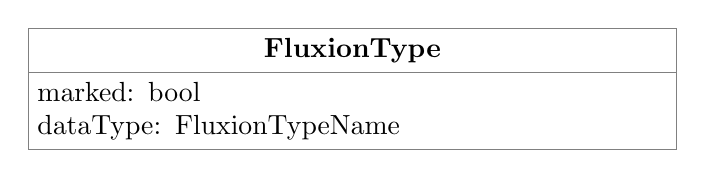
\begin{tikzpicture}
	\begin{class} [text width = 8cm]{FluxionType}{0,0}
		\attribute{marked: bool}
		\attribute{dataType: FluxionTypeName}
	\end{class}
\end{tikzpicture}
\end{center}
\caption{\code{FluxionType} struct, base for all types.}
\end{figure}

The \code{dataType} argument is of type \code{FluxionTypeName}, this is an enum typedef, and is one of: \code{Integer}, \code{Fraction}, \code{Matrix}, \code{Vector}, \code{Set}, \code{Sequence}, \code{Enumerable}

\subsection{Numeric Types}

When dealing with numbers, CFluxion has three internal representations, all of which inherit the \code{FluxionNumeric} typedef struct.

\begin{figure}[httb]
\begin{center}
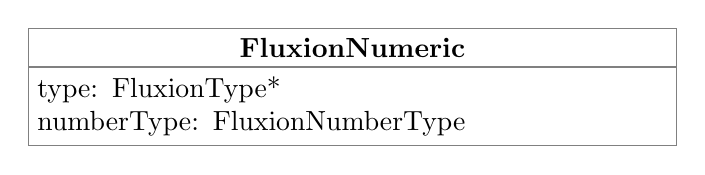
\begin{tikzpicture}
	\begin{class} [text width = 8cm]{FluxionNumeric}{0,0}
		\attribute{type: FluxionType*}
		\attribute{numberType: FluxionNumberType}
	\end{class}
\end{tikzpicture}
\end{center}
\caption{\code{FluxionNumeric} struct, base for all numbers.}
\end{figure}

The \code{FluxionNumberType} is a typedef enum, with the possible values \code{Integer}, \code{Number} and \code{Irrational}.\\

\code{FluxionInteger} struct typedef holds numbers smaller than $2^{32} - 1$, they are small enough that the benefit of introducing a more complex representation is outweighed by the cost this datatype comes with when it comes to simple arithmatic.

\begin{figure}[httb]
\begin{center}
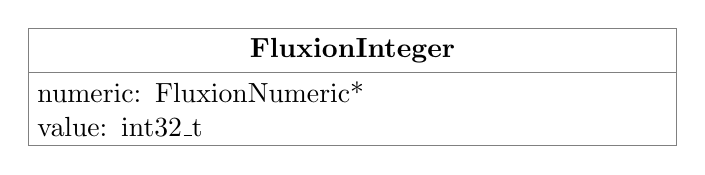
\begin{tikzpicture}
	\begin{class} [text width = 8cm]{FluxionInteger}{0,0}
		\attribute{numeric: FluxionNumeric*}
		\attribute{value: int32\_t}
	\end{class}
\end{tikzpicture}
\end{center}
\caption{\code{FluxionInteger} struct, for numbers that can fit \code{int32\_t}.}
\end{figure}

This more complex data structure is called \code{FluxionNumber}. Instead of holding the exact value like \code{FluxionInteger} does, \code{FluxionNumber} has four dynamically resizing arrays (pointers) each holding integers of type \code{uint64\_t}. These arrays are called \code{FluxionLongArray}, and this is an utility class.\\

These arrays, let us call them $S_1, S_2, S_3$ and $S_4$ are used to construct the actual numbers $i$ thusly:

\begin{equation}
i = \frac{x}{y} + \frac{z}{q}i = \frac{\sum S_1}{\sum S_2} + \frac{\sum S_3}{\sum S_4} i
\end{equation}

As can be seen, each list holds the prime factors of $x, y, z$ and $q$.\\

We are saving one bit here by using \code{uint64\_t}, however, we now need a way to express negativity, since negative numbers are allowed in Fluxion, this is achieved by putting a zero in $S_2$ or $S_4$. since zero cannot occur in these arrays, as that would create a divison by zero problem.

\begin{figure}[httb]
\begin{center}
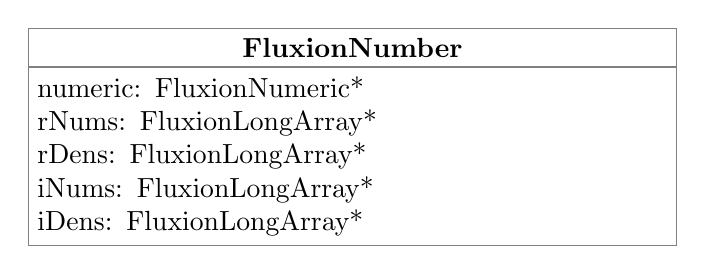
\begin{tikzpicture}
	\begin{class} [text width = 8cm]{FluxionNumber}{0,0}
		\attribute{numeric: FluxionNumeric*}
		\attribute{rNums: FluxionLongArray*}
		\attribute{rDens: FluxionLongArray*}
		\attribute{iNums: FluxionLongArray*}
		\attribute{iDens: FluxionLongArray*}
	\end{class}
\end{tikzpicture}
\end{center}
\caption{\code{FluxionNumber} struct, used for numbers.}
\end{figure}

Using a structure like this solves a couple of problems, first, it will avoid precision related issues ($0.1 + 0.2$ not equaling $0.3$, for instance). Second, it will make it possible for large numbers to be expressed easilly. And finally, this will make reduction significantly easier down the line.

\subsubsection{Irrational Numerals}

Since Irrational numerals are also reserved for use of the Fluxion language, there also exists a third value for numerical objects in Fluxion outside those numbers $x \not\in \mathbb{Q} \land x \in \mathbb{R}$. Most notably, three irrational numbers are reserved by the Fluxion standard, $e, \pi$ and $\tau$. These are represented by the \code{FluxionIrrational} class, there is also a helper enum typedef, \code{FluxionIrrationalType}, which is either \code{EULER}, \code{PI} or \code{TAU}.

\begin{figure}[httb]
\begin{center}
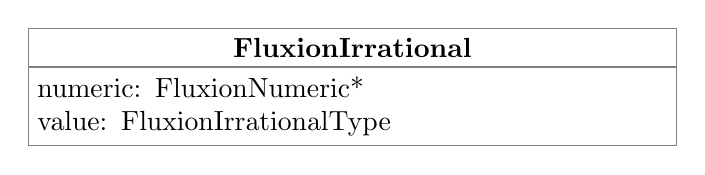
\begin{tikzpicture}
	\begin{class} [text width = 8cm]{FluxionIrrational}{0,0}
		\attribute{numeric: FluxionNumeric*}
		\attribute{value: FluxionIrrationalType}
	\end{class}
\end{tikzpicture}
\end{center}
\caption{\code{FluxionIrrational} struct, for $e, \pi$ and $\tau$.}
\end{figure}

\subsection{Matrices}

Matrices form an important part of mathemtics, and Fluxion, Matrices are represented using the base class \code{FluxionMatrix}, which has two subtypes, \code{Fluxion2Matrix} and \code{FluxionVector}. These subtypes are used for optimizing the memory usage of the classes.

\begin{figure}[httb]
\begin{center}
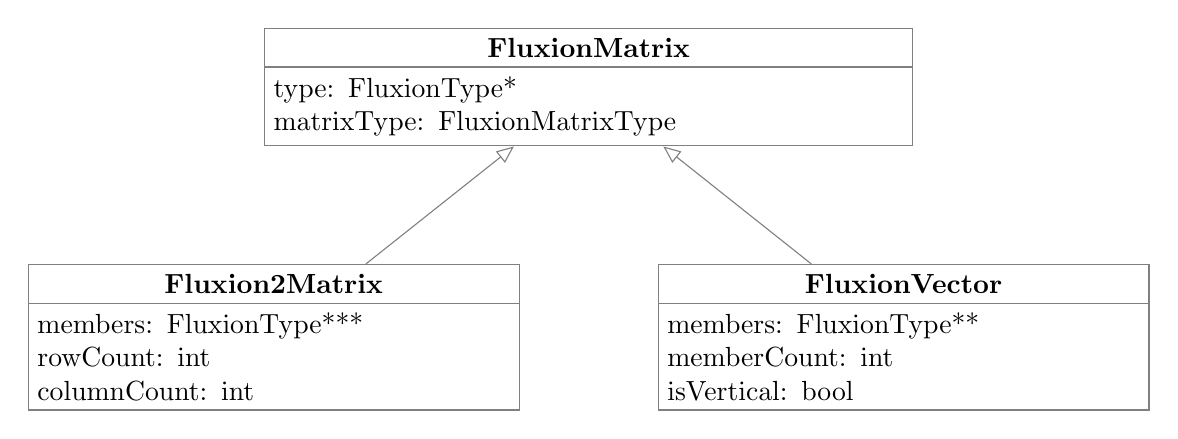
\begin{tikzpicture}
	\begin{class} [text width = 8cm]{FluxionMatrix}{0,0}
		\attribute{type: FluxionType*}
		\attribute{matrixType: FluxionMatrixType}
	\end{class}
	\begin{class} [text width = 6cm]{Fluxion2Matrix}{-4, -3}
		\inherit{FluxionMatrix}
		\attribute{members: FluxionType***}
		\attribute{rowCount: int}
		\attribute{columnCount: int}
	\end{class}
	\begin{class} [text width = 6cm]{FluxionVector}{4, -3}
		\inherit{FluxionMatrix}
		\attribute{members: FluxionType**}
		\attribute{memberCount: int}		
		\attribute{isVertical: bool}	
	\end{class}
\end{tikzpicture}
\end{center}
\caption{\code{FluxionMatrix} and its subtypes.}
\end{figure}

Observe that we can just use pointers here rather than any sort of dynamically allocated array since the size of vectors, and matrices, are known at compile time.

\subsection{Sets \& Sequences}

Despite being the same type, infinite sets differ significantly from finite ones. Actually, infinite enumarables, differ from infinite sets too, despite technically being a subtype of them, so much so same type can be used to represent both them and Sequences, which are \textbf{not} sets. But sometimes, sets and sequences can be auto-cast to each other.\\

This interchangableness of the type causes a unique situation, despite Enumerables are subtypes of Sets and Sequences are another type entirely in the Fluxion standard, CFluxion uses an enum typedef \code{FluxionColType} for collections, that takes one of three values \code{InfiniteSet}, \code{FiniteSet} and \code{Sequance}. It also uses a base typedef for all of them \code{FluxionCollection}\\

\begin{figure}[httb]
\begin{center}
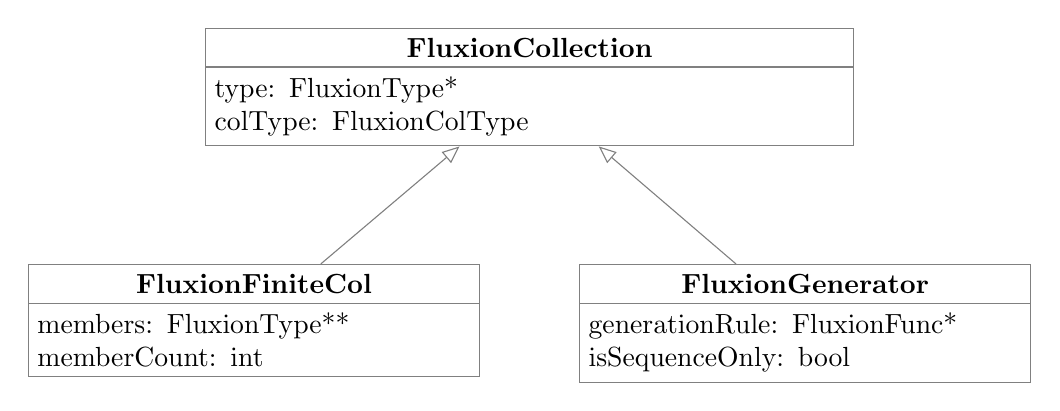
\begin{tikzpicture}
	\begin{class} [text width = 8cm]{FluxionCollection}{0,0}
		\attribute{type: FluxionType*}
		\attribute{colType: FluxionColType}
	\end{class}
	\begin{class} [text width = 5.5cm]{FluxionFiniteCol}{-3.5, -3}
		\inherit{FluxionCollection}
		\attribute{members: FluxionType**}
		\attribute{memberCount: int}
	\end{class}
	\begin{class} [text width = 5.5cm]{FluxionGenerator}{3.5, -3}
		\inherit{FluxionCollection}
		\attribute{generationRule: FluxionFunc*}
		\attribute{isSequenceOnly: bool}
	\end{class}
\end{tikzpicture}
\end{center}
\caption{\code{FluxionCollection} and its subtypes.}
\label{fig:collections}
\end{figure}

Observe in Figure \ref{fig:collections} that the generation rules for classes are normal Fluxion functions. \code{isSequenceOnly} is used for determining which operations are allowed on sequences. Also observe that the \code{FluxionFiniteCol} has a set number of members, as we also know the number of members of a sequence in compile time, \textit{and} Fluxion's collections are immutable.

\subsection{Operations}

Operations are, surprisingly, also types in Fluxion. The \code{FluxionOperation} struct typedef also inherits from \code{FluxionType}. And uses a helper enum typedef, \code{FluxionOpType}. Each enum represents a specific symbol. All operations are converted to a binary equivalent, for instance \code{- (x + 1)} is converted to \code{(-1) * (x + 1)}.

\begin{figure}[httb]
\begin{center}
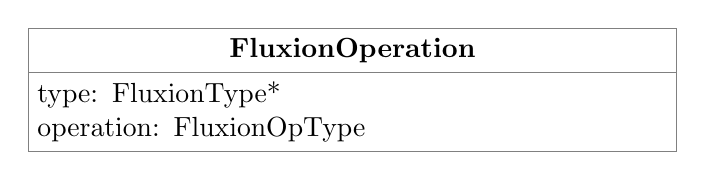
\begin{tikzpicture}
	\begin{class} [text width = 8cm]{FluxionOperation}{0,0}
		\attribute{type: FluxionType*}
		\attribute{operation: FluxionOpType}
	\end{class}
\end{tikzpicture}
\end{center}
\caption{\code{FluxionOperation} struct, representing an operation.}
\end{figure}

\subsection{Names \& Function Calls}

A Name is a variable name appearing inside an expression prior to binding. Function calls are also special names.\\

\begin{figure}[httb]
\begin{center}
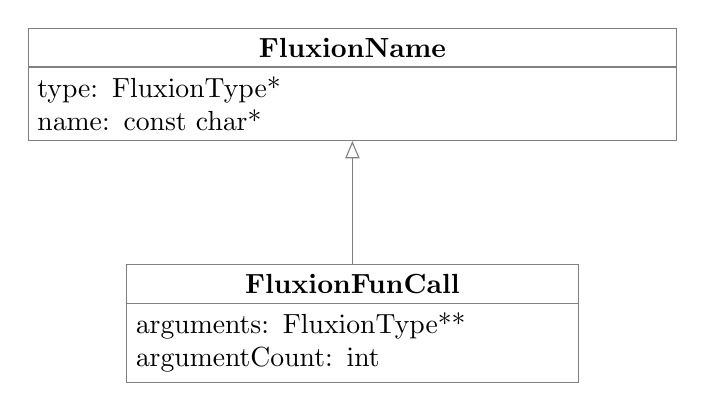
\begin{tikzpicture}
	\begin{class} [text width = 8cm]{FluxionName}{0,0}
		\attribute{type: FluxionType*}
		\attribute{name: const char*}
	\end{class}
	\begin{class} [text width = 5.5cm]{FluxionFunCall}{0,-3}
		\inherit{FluxionName}	
		\attribute{arguments: FluxionType**}
		\attribute{argumentCount: int}
	\end{class}
\end{tikzpicture}
\end{center}
\caption{\code{FluxionName} and \code{FluxionCall}, representing variables.}
\end{figure}

Although the argument count can be got from the actual function once the name is bound, the posibility of an erronous call means that the argument count must still be kept inside the body as well.

\pagebreak
\subsection{Expression}

Expressions are also \code{FluxionType}s, since they can appear inside function calls and alike. To be fair, this is actually because of the reverse, the Fluxion standard says the literals or variables of the other types by themselves are Expressions, but this is easier to implement.\\

The Expressions are, trees, more than that, they are binary trees. Since all of our operations are binary, and those types that are not operations can only apear in leaves of our tree.

\begin{figure}[httb]
\Tree [.\code{+} [.\code{/} \code{12} \code{2} ] [.\code{*} \code{3} \code{3} ] ]
\caption{Expression tree for \code{12/2 + 3 * 3}}
\label{fig:tree}
\end{figure}

As can be seen in Figure \ref{fig:tree}, expression trees also adhere to the precedence of the operations. Each expression is evaluated by evaluating the operation on its left storing the result in a variable $l$, then evaluating the expression on its right storing the result in a variable $r$, and then performing the apporiprate operation on them (depending on the operation) and returning the result $f(l, r)$.\\

Expressions are stored using a tree structure with an associative array, where, the root node is at index 1, and for each node in index $n$, 
its right node is in $2n$, and its left node is in $2n - 1$.\\

\begin{figure}[httb]
\begin{center}
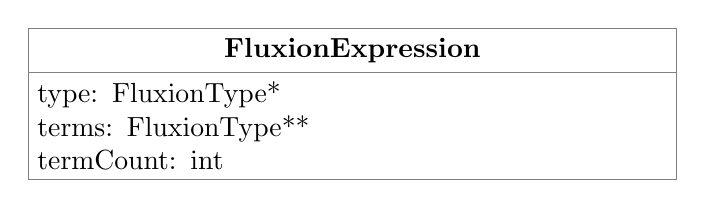
\begin{tikzpicture}
	\begin{class} [text width = 8cm]{FluxionExpression}{0,0}
		\attribute{type: FluxionType*}
		\attribute{terms: FluxionType**}
		\attribute{termCount: int}
	\end{class}
\end{tikzpicture}
\end{center}
\caption{\code{FluxionName} and \code{FluxionCall}, representing variables.}
\end{figure}

Again, since each token will compile to a set number of oprations, we know exactly how many terms there are. There are a few things to make sure while compiling an expression from its tokens. The first is to make sure the tree itself is balanced and second, is to make sure the order of precedence is preserved, the tree must be formed such that no operation of higher precedence will occur on a higher level of three than an operation with a lower precedence. To achieve these goals, we wil make two passes on the expression.\\

The first pass, we will extend any unary operation to its binary equivalent.

\end{document}